\documentclass[master=mai, masteroption=ecs]{kulemt} 
% \documentclass[master=ecws, masteroption=ai]{kulemt}
\setup{title={An Information Theoretical Approach to EEG Source-Reconstructed Connectivity},
  author={Axel Faes},
  promotor={Prof.\,dr.\,ir.\ Marc Van Hulle},
  assessor={Mansoureh Fahimi\\Prof.\,dr. Daniele Marinazzo},
  assistant={Mansoureh Fahimi}}
% The following \setup may be removed entirely if no filing card is wanted
\setup{filingcard,
  translatedtitle=,
  udc=681.3*I20,
  shortabstract={
Determining how distinct brain regions are connected and communicate with each other will shed light on how behaviour emerges. In EEG studies, interpreting connectivity measures can be problematic, due to the high correlation between signals recorded from the scalp surface, a result of the volume conductance of the scalp and skin. Therefore, meaningful connectivity patterns can be measured only from the from the spatiotemporal distribution of localised cortical sources, generally referred to as source reconstruction. Still, spurious connectivity issues may persist in source reconstructed EEG data, rendering it vital to choose an appropriate measure of connectivity.
This thesis takes an information theoretical approach, which concerns model-free, probability based methods such as Conditional Mutual Information, Directed Information, and Directed feature information. We will investigate how these measures are affected by volume conduction, using as ground truth connectivity between simulated cortical sources in the brainstorm toolbox. In order to validate our methods further, these tools will also be compared with their statistical counterparts such as partial correlation, granger causality and dynamic causal modelling.
The student will start by studying state-of-the-art literature concerning source localisation and the problem of volume conduction. The student will also familiarise himself with information theoretical measures of brain connectivity. Afterwards, these measures will be applied to high density EEG datasets provided by the lab of computational neuroscience, but also to simulated source activity as a validation. The novelty lies in the usage of these information theoretical algorithms for source-reconstructed activity.
}}

% Choose the main text font (e.g., Latin Modern)
\setup{font=lm}

%% Some recommended packages.
\usepackage{booktabs}   %% For formal tables:
                        %% http://ctan.org/pkg/booktabs
\usepackage{subcaption} %% For complex figures with subfigures/subcaptions
                        %% http://ctan.org/pkg/subcaption

\usepackage{array}
\usepackage{mathpartir}
\usepackage{xspace}
\usepackage{stmaryrd}
\usepackage{amsmath}
\usepackage{listings}
% \usepackage{newtxmath}
\usepackage{float}
\usepackage{pdfpages}
\usepackage{bm}

\usepackage{todonotes}

%% Tikz Needed packages
\usepackage{pgfplots}
\pgfplotsset{width=7cm,compat=1.8}
\usepackage{pgfplotstable}
\renewcommand*{\familydefault}{\sfdefault}

% Finally the hyperref package is used for pdf files.
% This can be commented out for printed versions.
\usepackage[pdfusetitle,colorlinks,plainpages=false]{hyperref}

% \input{tex/00-macros}

\lstset{
  columns=fullflexible,
  frame=single,
  breaklines=true,
  postbreak=\mbox{\textcolor{red}{$\hookrightarrow$}\space},
}

\begin{document}

\renewcommand{\prefacename}{Acknowledgements}
\begin{preface}
  This thesis has been quite a long journey. I was able to get invested into an interesting field of research and learn a lot of new things. Both about research, and about myself. \\ 
\\
  I would like to thank everybody who kept me busy and supported me the last year. I would also like to thank the jury for reading the text. 
\end{preface}

\tableofcontents*

\setlength{\parindent}{0pt}
\setlength{\parskip}{1em}

\begin{abstract}
Determining how distinct brain regions are connected and communicate with each other will shed light on how behaviour emerges. In EEG studies, interpreting connectivity measures can be problematic, due to the high correlation between signals recorded from the scalp surface, a result of the volume conductance of the scalp and skin. Therefore, meaningful connectivity patterns can be measured only from the from the spatiotemporal distribution of localised cortical sources, generally referred to as source reconstruction. Still, spurious connectivity issues may persist in source reconstructed EEG data, rendering it vital to choose an appropriate measure of connectivity.

This thesis takes an information theoretical approach, which concerns model-free, probability based methods such as Conditional Mutual Information, Directed Information, and Directed feature information. We will investigate how these measures are affected by volume conduction, using as ground truth connectivity between simulated cortical sources in the brainstorm toolbox. In order to validate our methods further, these tools will also be compared with their statistical counterparts such as partial correlation, granger causality and dynamic causal modelling.
  
The student will start by studying state-of-the-art literature concerning source localisation and the problem of volume conduction. The student will also familiarise himself with information theoretical measures of brain connectivity. Afterwards, these measures will be applied to high density EEG datasets provided by the lab of computational neuroscience, but also to simulated source activity as a validation. The novelty lies in the usage of these information theoretical algorithms for source-reconstructed activity.
\end{abstract}

\listoffigures

% Now comes the main text
\mainmatter

\chapter{Introduction}
Within the field of computational neuroscience, extensive research is being done on the connectivity of brain regions. Understanding how distinct brain regions are connected can answer many different questions. It will shed light on how behaviour emerges. 

There are multiple ways to study brain connectivity. Brain connectivity can be studied on different levels, such as microscale or macroscale. Another question is what kind of connectivity is being measured. There is a distinction between the structural (or anatomical) connectivity and the functional connectivity. At the macroscale, functional connectivity can be measured with multiple imaging techniques. One popular imaging technique is EEG.

In EEG studies, interpreting connectivity measures can be problematic, due to the high correlation between signals recorded from the scalp surface, a result of the volume conductance of the scalp and skin. Therefore, meaningful connectivity patterns can be measured only from the from the spatiotemporal distribution of localised cortical sources, generally referred to as source reconstruction. Still, spurious connectivity issues may persist in source reconstructed EEG data, rendering it vital to choose an appropriate measure of connectivity.

This thesis takes an information theoretical approach, which concerns model-free, probability based methods such as Conditional Mutual Information and Directed Information. These methods are applied on real data, provided by the lab of computational neuroscience. This dataset contains source-reconstructed EEG data, recorded in an experiment revolving around semantic processing. 

The experiment focussed on two word categories: abstract words and concrete words. The data contains several brain regions of interest. The semantic processing of abstract and concrete words is slightly different. Some of the semantic processing is done in separate brain regions. There also is a region where semantic processing occurs in both the abstract and concrete experiments, in this thesis, this is called the common region.

\section{Research Questions}

From the motivation, there are two big aspects that this thesis deals with. There is information theory and source-reconstructed EEG Data. The novelty of this thesis lies in the usage of these information theoretical algorithms for source-reconstructed EEG data.

\begin{itemize}
\item How can information theoretical measures be applied to source-reconstructed EEG Data?
\item Which observations can be made by applying these information theoretical measures on a high density EEG dataset provided by the lab of computational neuroscience?
\end{itemize}

\section{Approach}

The goal of this thesis, as well as it's main contribution, is to apply information theoretical measures on a high density EEG dataset provided by the lab of computational neuroscience. There are two steps to accomplish this. First, an implementation has to be made that can perform an information theoretical analysis of source-reconstruted EEG Data. Secondly, the information theoretical measures are applied to a dataset. Important in this step is to decide how to analyse the data.

\begin{enumerate}
\item Study of the relevant state-of-the-art literature and theoretical background. This includes source reconstruction, brain connectivity and information theory.
\item Development of framework for information theoretical analysis of source-reconstruted EEG Data.
\item Application of information theoretical measures to high density EEG dataset provided by the lab of computational neuroscience.
\end{enumerate}

\section{Results}

The main novelty lies in the application of information theoretical algorithms for source-reconstructed EEG data. Behind this novelty, there are several different deliverables that made it possible to reach the goal of this thesis. 

The implementation of the information theoretical algorithms is a first result of this thesis. The implementation is the backbone behind the thesis. The implementation consists out of three parts. There is the data conversion, which converts the source-reconstructed EEG data into multiple format. Secondly, methods for calculating the correct amount of bins to discretize the continious data have been implemented. 

Finally, the actual information theoretical equations have been implemented. The implementation is developed to be of general use, meaning that it isn't too difficult to convert the implementation into an open source connectivity package.

A second result of this thesis is the actual analysis of the high density EEG dataset provided by the lab of computational neuroscience. The main conclusion made in the analysis of the EEG dataset, is that, within the common region, the actual semantic processing is quite different between the semantic processing of abstract words and the semantic processing of concrete words.

\section{Structure of the Thesis}

Chapter~\ref{source-reconstruction} discusses source reconstruction. It starts by explaining what source reconstruction entails and why it is important. Afterwards, an explanation is given about the reasons that spurious connectivity issues may still persist in source reconstructed EEG data.

Chapter~\ref{connectivity} gives a background of brain connectivity and volume conduction. this chapter hightlights the different kinds of connectivity and brievely discusses them.

Chapter~\ref{information-theory} provides a background about information theory. This chapter starts by explaining the concept of information entropy. Using this concept, the different aspects from information theory are discussed, including joint entropy, mutual information, multivariate methods and directed information. Finally, this chapter details methods on how to use information theory on continuous data.

Chapter~\ref{eeg-experiment} details the experiment that generated the data which this thesis analyses. This chapter starts by detailing the reasons behind the experiment and then details the experiment itself.

Chapter~\ref{evaluation} will go in depth into the actual analysis that has been done on the data. The binning and the different analysis experiments are described. 

Chapter~\ref{implementation} goes in depth into the source code that has been developed for the analysis. There are several important aspects to be discussed about the source code, such as the programming language and the implementation of the equations.

Chapter~\ref{related} brievely discusses some related work. More specifically, granger causality is detailed. Chapter~\ref{future-work} details several interesting directions we can take this research. Considering the conclusion of this thesis, that information theoretical algorithms work well on source-reconstructed EEG data, many new paths open for further investigation. Finally, chapter~\ref{conclusion} concludes the thesis.

\chapter{Source Reconstruction}\label{source-reconstruction}
Source reconstruction refers to the localisation of the electrical activity of the brain. In the case of this thesis, we are referring to EEG source localization, which is also called the reverse problem. Electrical activity within the brain is measured on the scalp using EEG electrodes. This is the forward problem. The reverse problem maps the measurements from the EEG electrodes back into the brain. 

\section{Reverse Problem}

Figure~\ref{source-local-img} visualizes the reverse problem. This is an ill-posed problem. EEG electrodes measure the scalp, in effect measuring a 2D grid. However, the brain is a 3D object. This means that information is inherently lost when EEG is used. One of the consequences is there are many different solutions to the reverse problem. 

\begin{figure}[!htb]
\caption{EEG Source Localisation \cite{source-loc-img}.}
\label{source-local-img}
    \centering
    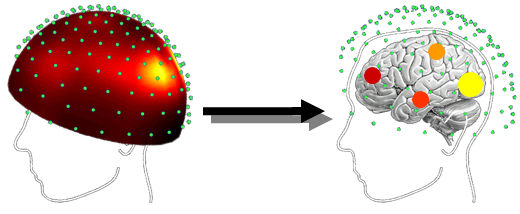
\includegraphics[width=\textwidth]{fig/source_recon}
\end{figure}

Equation~\ref{reverse} represents source localisation. $X$ represents the scalp recorded EEG activity. $S$ represents the electrical sources within the brain, a current density vector. $L$ represents the head volume conductor model. The reverse problem is about finding $S$, this is represented in equation~\ref{reverse2}.

\begin{equation}\label{reverse}
X = LS + n
\end{equation}

\begin{equation}\label{reverse2}
O(S) = min||X - LS||^2 
\end{equation}

\section{Head Volume Conductor Model}

Several different head volume conductor models can be used. The two most popular are the simple head models and the realistic head models. Simple head models modle the brain as a single sphere with a couple layers. This model also assumes a uniform medium within the brain. Using a simple head model is fast and simple. However, it is not accurate. 

The realistic head model is an accurate model, but it is computationally much more expensive. Different techniques are used to construct a head model such as finite element or finite boundary techniques. 

\section{Dipoles}

The electrical sources within the brain are also called dipoles. The inverse problem is essentially about deciding how many dipoles there are and where these dipoles are located. 

There are practical limits to the number of dipoles that can be used. One of the most important limits is the spatial resolution of EEG. EEG can only measure electrical activity with a certain accuracy. This is due to the fact that the electrical activity is measured on the scalp. 

\section{Algorithms}

There are different kind of algorithms used to solve the inverse problem. There is dipole fitting, which involves only a small number of dipoles. The locations, orientations, and magnitudes of these dipoles needs to be calculated. For some experiments, this method can be good enough, since a single dipole can account for 80\% of all electrical activity.

Then there are nonadaptive distributed-source imaging methods and adaptive distributed-source imaging methods. The idea of distributed-source imaging is that thousands of dipoles are placed within the brain on fixed locations with fixed orientations. This leaves only the magnitude to be computed. This is done by assigning electrode weights to each dipole.

Nonadaptive methods compute these electrode weights based on the electrode locations. This means that the weights are fixed over time and frequency. sLORETA is a commonly used nonadaptive inverse-source imaging technique. The provided data used in this thesis has also been source-reconstructed using sLORETA.

Nonadaptive methods are relatively fast to compute, are applicable to single time points and their result looks like FMRI activation maps. However, there are also some disadvantages. One issue is that the electrode weights are not computed using statistical properties of the data. 

Adaptive distributed-source imaging have a different way of computing the electrode weights. The recorded data is also used to compute the weights. The weights are not fixed over time and frequency. The accuracy of adaptive methods is often quite high, but they are much more complicated with many more parameters to be set. 

\section{Practical Limits}

Within a simulated environment, high spatial localization accuracy can be obtained. However, in practive, there are many issues. There are always uncertainties regarding electrode positions, brain anatomy, head movement and scalp conductivity. This means that spatial accuracy is often a few centimeters in size. The smallest voxels which are created by source reconstruction are typically 5-10 mm$^3$ in size. 

Without knowledge of the inverse problem, it might seem that source reconstruction is not a big deal. It might even seem to only bring advantages, since you can work within the actual cortical areas. However, source reconstruction comes with its fair share of problems and inaccuracies. 

Within the context of this thesis, knowledge of the inverse problem is essential. While the data was already source-reconstructed, for the reasons above, it is important to know the inverse problem. 

\chapter{Brain Connectivity}\label{connectivity}
The human brain is anatomically a conglomeration of different brain regions. Functionally, the human brain is a giant network of specialised units connected by dynamically configurable communication pathways. \cite{faes2012methodological}

There are several reasons why scientists would want to measure the way the brain is connected. Understanding brain connectivity aids our knowledge of the working of the brain. It allows us to better understand sensorimotor and cognitive tasks that are performed. This can lead to improved diagnosing of various diseases such as aphasia. \cite{horwitz2003elusive}

A connectivity analysis refers to any analysis where multiple signals are utilised at the same time. The signal can represents several different sources. The signals could be the recordings from different electrodes or, in the case of this thesis, the source-reconstructed EEG data. 

\section{Connectivity Measures}

Different connectivity measures can highlight different aspects about the connectivity. This means that there is not one superior connectivity method. The different connectivity measures are: \cite{friston2011functional, cohen2014analyzing}

\begin{itemize}
\item Phase-Based Connectivity
\item Power-Based Connectivity
\item Cross-Frequency Coupling
\item Graph Theory
\item Granger Causality
\item Information Theory
\end{itemize}

\subsection{Phase-based Connectivity}

Phase-based connectivity analyses utilise the phase differences between different signals. This is a very popular connectivity measure and this is partly because it has a strong neurophysiological interpretation. The timing of neural populations, as measured through phase, become synchronized. This method is computationally fast, does not make many assumptions on the data and is insensitive to time lag. However, it relies on precise temporal relationships.

\subsection{Power-based Connectivity}

Power-Based Connectivity analyses utlise time-frequency power correlations. These correlations are computed accross time or over trials. Power-Based Connectivity analyses are fairly resistant against temporal noise.

\subsection{Cross-Frequency Coupling}

Cross-Frequency Coupling is a statistical relationship between signals in different frequency bands. When utilised on electrodes, it can infer local connectivity when measured at a single electrode. With multiple electrodes, longer-range connectivity can be inferred. One advantage is that findings can be linked across species. Cross-frequency coupling is also very strong at identifying task-related high-frequency power. Computationally speaking, there are some disadvantages to cross-frequency coupling. The search space is huge, which makes it computationally very expensive.

\subsection{Graph Theory}

Graph Theory is a mathematical framework for studying graphs. A graph, containing vertices and edges, can be used to model networks. These networks can be models for brain connectivity. When electrode signals are used, each node can represent an electrode and connectivity is represented by edges. Graph-theoretical analyses are often easy to interpret. Graph theory presents a generic framework to analyse networks, making it easy to apply the same analyses to different kinds of data. The main task becomes the construction of a network. Graph theory is relatively new in the context of computational neuroscience. This makes graph theory an interesting research direction, but this is also a disadvantage. Since graph theory within computational neuroscience isn't as well established, it can be difficult to compare findings to different studies.

\subsection{Granger Causality}

Granger Causality is a statistical method that utilises signal variance. It tests whether variance from one signal can predict variance in another signal at a certain point in time. One big advantage to granger causality is that it can find directional connectivity. It can ignore simultaneous connectivity. This makes it less susceptible to volume conduction. Granger causality is a computationally expensive method to perform. \cite{bressler2011wiener}

\subsection{Information Theory}

Information theory is the main focus of this thesis. It is a simple, yet flexible and robust method for computing connectivity. One useful aspect from information theory is mutual information. Mutual information computes shared information between two variables. This computation is based on the (joint) distributions of values within variables. Information theory has several advantages. It can detect multiple kinds of relationships between different signals. It can detect both linear and non-linear relationships. Information theory also contains many different constructs which are useful for a connectivity analysis. Mutual information is one of them. Another is multivariate generalisations of mutual information, which can work with more than two signals. Channel-coding theory can be used for signal transmission integrity. 

Mutual information is, by far, the most popular method from information theory. One disadvantage is that mutual information does not provide any information on what kind of relationship there is between variables. Information theory is generally defined for discrete distributions, with different techniques to discretize continuous data. However, the method and the chosen parameters for discretizing continuous data have a big effect on the computed results. Information theory is generally also a computationally expensive operation to perform. Finally, there are no clear neurophysiological interpretations for information theoretical constructions. Information theory is discussed much more in-depth in the following chapter, chapter~\ref{information-theory}.

\section{Connectivity Interpretation}

There are several key aspects to keep in mind when interpreting results from a connectivity analysis. Different connectivity measures may or may not take these aspects into consideration. In order to provide a proper connectivity analysis, these key aspects and the properties of the connectivity measures need to be known.

Typically, two different signal are not fully in sync. When an analysis is performed on the signal from multiple electrodes, there may be a phase lag between these electrodes. Most connectivity measures do not take this phase lag into consideration. This does not mean that that these connectivity measures cannot be used, as long as the phase lag is consistent. \cite{horwitz2003elusive}

Figure~\ref{timelag} shows a second key aspect. In this example, region C is connected with A and B. Because C$\rightarrow$A is faster than C$\rightarrow$B, it may appear that there is a phase lag, even though there is no causal or direct relation between A and B.

\begin{figure}[!htb]
\caption{Time Lag \cite{cohen2014analyzing}.}
\label{timelag}
    \centering
    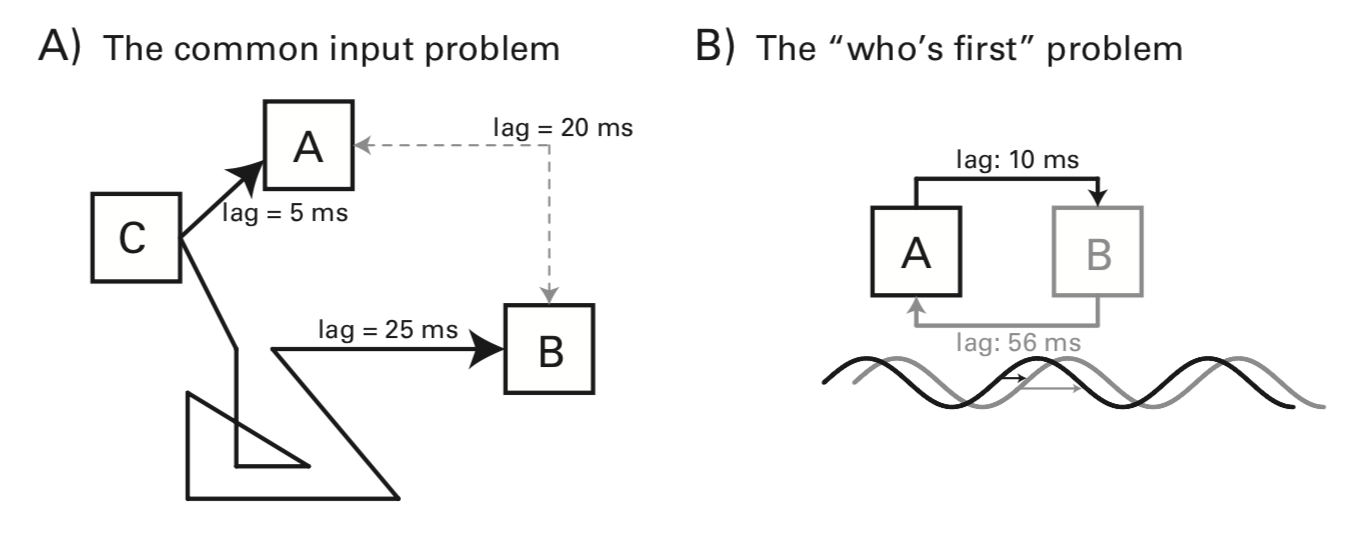
\includegraphics[width=\textwidth]{fig/timelag}
\end{figure}

\section{Volume Conduction}

The head volume conductor model, discussed in chapter~\ref{source-reconstruction}, is quite interesting. The brain conducts electrical activity, this is how the electrical activity can be measured on the scalp. Volume conduction refers to this process of conducting electrical activity through a medium. \cite{brunner2016volume}

Figure~\ref{conduction} shows several problems that the reverse problem has to deal with. In situation A, there would be no problem. In this situation, every EEG electrode measures one and only one electrical source within the brain. However, this is not what happens in reality. 

\begin{figure}[!htb]
\caption{Volume Conduction \cite{cohen2014analyzing}.}
\label{conduction}
    \centering
    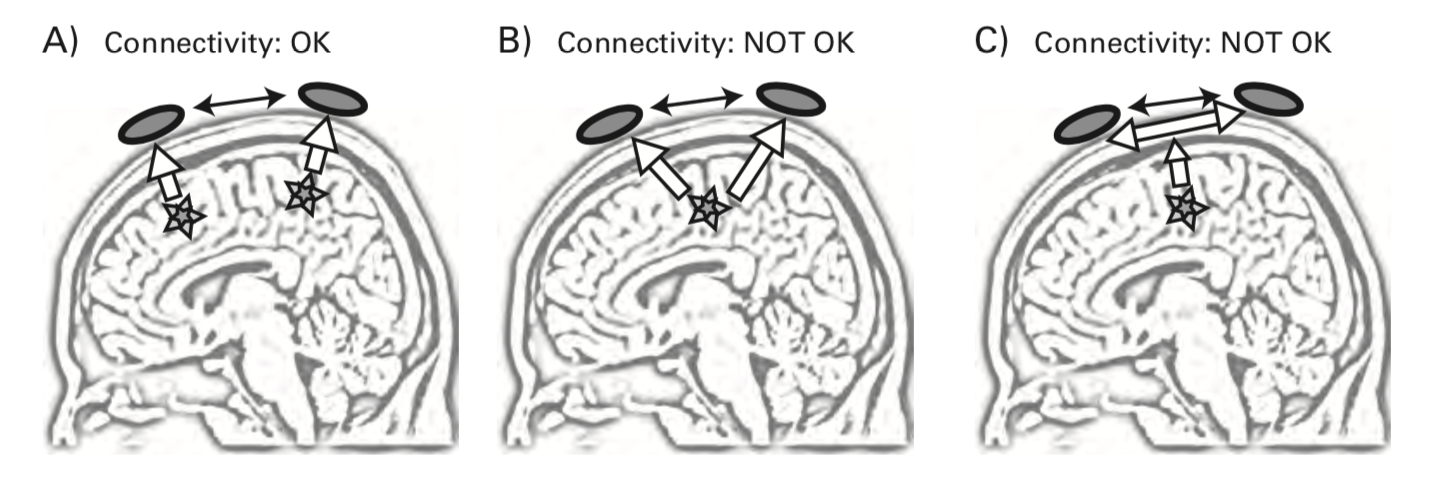
\includegraphics[width=\textwidth]{fig/conduction}
\end{figure}

Reality is a combination of situations B and C \cite{brunner2016volume}. Situation B shows that electrical sources in the brain generate large electromagnetic fields which are recorded by more than one EEG electrode. Situation C shows that the scalp also conducts electricity. These two situations have a big effect on connectivity measures. 


\chapter{Information Theory}\label{information-theory}
% \section{Information Theory}
Information theory provides us the tools to study the information processing capabilities of different systems. These systems include computers, artificial intelligence and also the brain. The story of Information Theory begins with Shannon who provided the tools to estimate information \cite{shin1949mathematical}. The most fundamental aspect of information theory is the concept of the 'bit'. 

As a standard, information theory deals with 'bits'. One bit of information represents a choice between two equally probable options. A perfectly balanced coin toss contains one bit of information. It has 50\% chance of landing on head and 50\% chance of landing on tails. A bit is a measure of information and a measure of uncertainty. Thus uncertainty and information are tightly intertwined. If we are completely certain about a certain event, there is no information to be gained. 

This chapter will cover the most important aspects of information theory. First and formost, this means discussing entropy. Once we have an understanding of entropy, extensions can be discussed. These include joint entropy and conditional entropy. With these tools, we can go into the area of mutual information, which plays an important role in this thesis. Another important aspect is the generalisation into multivariate systems and dealing with continuous (as opposed to discrete) systems. Finally, some explanation is provided of coding theory and cybernetics.

\section{Entropy}

The next step is entropy. There are different kinds of entropy, such as thermodynamic entropy. Here, we are talking about information entropy. Information entropy is the average uncertainty associated with a random variable. In other words, information entropy is the average rate of information from a random or stochastic variable. 

In order to calculate the entropy, we require some discrete random variable X, with ${x_1 ... x_n}$ the different values from X. $P(x)$ is the probability mass function. The entropy $H(X)$ can be calculated as:

\begin{equation}
H(X) = -\sum_{i=1}^{n}P(x_i)log_2(P(x_i))
\end{equation}

Interesting to note is that $log_2(P(x_i))$ is the information about value $x_i$. This formula can be extended into the conditional entropy of two events $X$ and $Y$. The entropy $H(X|Y)$ is the entropy of random variable X given that the outcome of Y is known.

\begin{equation}
H(X|Y) = \sum_{i,j}P(x_i, y_j)log_2(\frac{P(y_j)}{P(x_i, y_j)}) = -\sum_{i,j}P(x_i, y_j)log_2(\frac{P(x_i, y_j)}{P(y_j)})
\end{equation}

If random variables X and Y are independent of eachother, then $H(X|Y) = H(X)$. If the variables are completely independent, knowing anything about Y, will not change anything we know about X. Similarly, if $H(X|Y) = 0$, then X is completely determined by Y. 

The rule of Bayes is also applicable to conditional entropy:

\begin{equation}
H(X|Y) = H(Y|X) + H(Y) - H(X)
\end{equation}

\section{Joint Entropy}

$H(X)$ and $H(X|Y)$ are basic notions of information measures. Figure~\ref{entropy} visualises the notion of entropy. This figure also contains two information measures that are not yet described, $I(X,Y)$ and $H(X,Y)$. Respectively, they are the mutual information and the joint entropy.

\begin{figure}[!htb]
\caption{Venn diagram for information measures.}
\label{entropy}
    \centering
    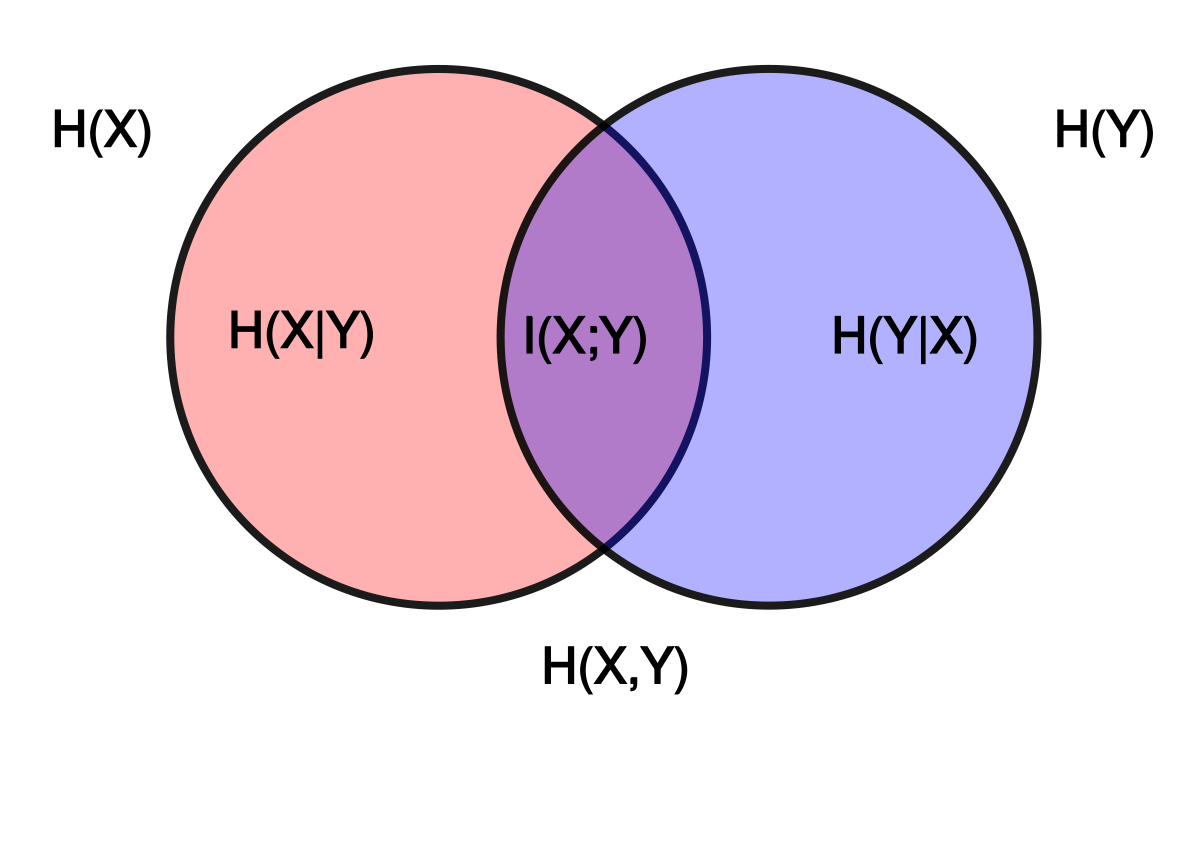
\includegraphics[width=0.8\textwidth]{fig/entropy}
\end{figure}

In the figure, $H(X,Y)$ is the complete information content of X and Y. Using the following equation, we can calculate $H(X,Y)$:

\begin{equation}
H(X,Y) = -\sum_{i=1}^{n}\sum_{j=1}^{m}P(x_i, y_j)log_2(P(x_i, y_j))
\end{equation}

Using figure~\ref{entropy}, we can see some interesting relations. $H(X,Y)$ is related to $H(X|Y)$ and $H(X)$:
\begin{equation}\label{joint}
H(X,Y) = H(X|Y) + H(Y)
\end{equation}

This can be validated:
\begin{align*}
H(X,Y) &= -\sum_{i=1}^{n}\sum_{j=1}^{m}P(x_i, y_j)log_2(P(x_i, y_j))\\
&= -\sum_{i=1}^{n}\sum_{j=1}^{m}P(x_i, y_j)log_2(P(y_i)P(x_i | y_j))\\
&= -\sum_{i=1}^{n}\sum_{j=1}^{m}P(x_i, y_j)log_2(P(y_i))-\sum_{i=1}^{n}\sum_{j=1}^{m}P(x_i, y_j)log_2(P(x_i | y_j))\\
&= -\sum_{j=1}^{m}P(y_j)log_2(P(y_i))-\sum_{i=1}^{n}\sum_{j=1}^{m}P(x_i, y_j)log_2(P(x_i | y_j))\\
&= H(Y) + H(X|Y)
\end{align*}

This relation is useful for the actual implementation of information theoretical algorithms. An important note about entropy, conditional entropy and joint entropy is that they are non-negative. It would not make sense for an random variable to have a negative information content. Joint entropy is also always greater or equal to individual entropy and joint entropy is smaller or equal to the sum of individual entropies.

\begin{equation}
H(X) \ge 0
\end{equation}

\begin{equation}
H(X|Y) \ge 0
\end{equation}

\begin{equation}
H(X,Y) \ge 0
\end{equation}

\begin{equation}
H(X,Y) \ge H(X)
\end{equation}

\begin{equation}
H(X,Y) \le H(X) + H(Y) 
\end{equation}

\section{Mutual Information}
Mutual information is the amount of information that is common between two variables. Figure~\ref{entropy} shows the mutual information as the intersection between $H(X)$ and $H(Y)$. The figure also shows how mutual information can be computed. The individual entropies are summed and the joint entropy is subtracted. Another equal interpretation of mutual information is that mutual information measures the reduction in uncertainty or information when we observe one of the variables.

\begin{equation}
I(X,Y) = H(X) + H(Y) - H(X,Y)
\end{equation}

\begin{equation}
I(X,Y) = H(X) - H(X|Y)
\end{equation}

Mutual information can also be calculated using the probability mass functions directly. In this case we get:

\begin{equation}
I(X,Y) = \sum_{i=1}^{n}\sum_{j=1}^{m}P(x_i, y_j)log_2(\frac{P(x_i, y_j)}{P(x_i)P(y_j)})
\end{equation}
    
While mutual information does show whether there is a relationship or correlation between two variables, it does not give information about the "shape" of the relationship. Making the analogy with figure~\ref{entropy}, mutual information shows how much overlap there is, but it does not explain anything else. Mutual information makes no assumptions of what the distribution of the variables X and Y is like. 

Mutual information, like entropy, is non-negative. Additionally, just like there is conditional entropy, there is also conditional mutual information. Conditional mutual information indicates the mutual information given another variable is given:

\begin{equation}
I(X,Y|Z) = \sum_{k=1}^{o}\sum_{i=1}^{n}\sum_{j=1}^{m}P(x_i, y_j, z_k)log_2(\frac{P(x_i, y_j z_k)P(z_k)}{P(x_i, z_k)P(y_j z_k)})
\end{equation}

\section{Multi-Variate Information Theory}
In the previous sections, information theory has been observed through a bivariate lens. These methods can be generalised to multivariate variations. When comparing different brain regions, we do not want to restrict ourselves to a bivariate case.

Joint entropy can be easily extended to a multivariate case. In the bivariate case, the joint probability mass function was used and a summation over both random variables was done. The multivariate case simply generalises this equation:

\begin{equation}
H(X_1, ..., X_n) = -\sum_{x_1}...\sum_{x_n}P(x_1,...,x_n)log_2(P(x_1,...,x_n))
\end{equation}

Equation~\ref{joint} can also be extended into a multivariate case. In this case, we get:

\begin{equation}
H(X_1, ..., X_n) = -\sum_{k=1}^{n}H(X_k|X_{k-1},...,X_1)
\end{equation}

The multivariate case of conditional entropy becomes:

\begin{equation}
H(Y | X_1, ..., X_n) = H(Y, X_1, ..., X_n) - H(X_1, ..., X_n)
\end{equation}

Having extended the different forms of entropy into a multivariate case, we can make a multivariate method for mutual information. The multivariate mutual information becomes a recursive function:

\todo{add mutual information + conditional}

\section{Continuous Data}

\todo{explain that we have continuous data, not discrete}

\section{Coding Theory}

\section{Cybernetics}

\chapter{EEG Experiment}\label{eeg-experiment}
Applying information theoretical algorithms on a high density EEG dataset is the main focus of this thesis. The EEG dataset is provided by the lab of computational neuroscience of KU Leuven. In order to perform an analysis of a dataset, it is important to understand what kind of data we are dealing with.

This chapter discusses the experiment used to generate the dataset. The experiment and the reasons behind the experiment are introduced. Afterward the actual experiment is discussed. This starts with the an explanation of the EEG experiment itself and the paradigm. Afterwards the source localization is discussed. Finally, the final structure of the data is brievely discussed.

\section{Introduction}

The experiment resolves around the human brain's representation of semantic categories. By using high density EEG recordings, the semantic processing of words within the human brain was captured. Within the literature, there are several different theories and concepts that explain the representation of semantic categories within the human brain. The human brain is a complicated organ with many different cortical areas. Each theory focusses on different cortical areas and explain how they are involved with the representation of semantic categories. These theories have been further developed with the aid of different neuroimaging experiments. 

One of the most prominant theories of semantic word processing is the grounded cognition model. The model is also called the embodied cognition model. This model explains that semantic knowledge is kept within high-level perception and motor representation systems in the brain. 

This means that a word is comprehended based on modality-specific neural systems. In other words, elements such as visual and auditory features are used to define words. As an example, animate objects cluster in the more lateral aspect of the fusiform gyrus, whereas activations associated with inanimate or man-made objects cluster in the more medial aspect of the fusiform gyrus \cite{landrum2015clinvar}. There are other studies that show that damage to the brain's modal system creates category-specific deficits \cite{barsalou2003grounding, caramazza2003organization}. 

These deficits can be explained by using the grounded model, natural objects such as animals, vegetation, etc, are distinguished primarily from their visual semantic properties. On the other hand, man-made objects such as tools and vehicles are distinguished primarily by their function. This is also shown by fMRI and PET imaging studies \cite{devlin2002there}.

The grounded cognition model can be criticized from several aspects. Stimuli that are conceptual in nature are much more difficult to control, as the associated brain activity is almost completely subject-dependent \cite{kemmerer2015visual}. Most importantly, the grounded cognition model only explains features that are related to a physical object. More abstract concepts, such as concepts related to emotions, are not explained by the model. 

Looking at the difference in the processing of abstract and concrete words, there are some theories. The main theories are the dual coding theorem and the context availability theorem \cite{kounios1994concreteness, wang2010neural}. The dual coding theorem states that there are two separate systems within the brain, a nonverbal "imagery" system and a verbal "linguistic" system. The nonverbal system implement is very alike to the grounded cognition model. The verbal system is involved with the abstract nature of language.

The context availability theorem is quite different from the dual coding theorem. Rather than having two distinct systems, the context availability theorem states that the processing of concrete and abstract words never happen in isolation and that context is important. Context determines how words are processed. Concrete words are contextually related to their physical referents. Abstract words are more variable and are contextually related to previous experience. 

Neither theory has been proven or disproven by scientific literature. Most research into these theories have been done using functional neuroimaging techniques such as fMRI and PET, which is limited in terms of temporal resolution \cite{bookheimer2002functional}. EEG, by virtue of its excellent temporal resolution, has become popular to probe the brain's detailed processing of objects and words. Several studies using EEG/ERP recordings have successfully distinguished different word categories. This has been done on different stages of semantic processing \cite{hauk2006time}. One disadvantage to using EEG is the low spatial resolution, which makes it fall short in detecting cortical network activiation differences. 

In the experiment described in this chapter, high density EEG recordings were used to capture the fast dynamics involved in semantic processing. The neural activity has been localized on the cortex with an accuracy in the range of millimetres and milliseconds. This provides an interesting and unique opportunity to analyse the activity during the semantic processing of abstract and concrete words.

\section{Materials and methods}

The experiment was done in a sound-attenuated, darkened room with a constant temperature of 20 degrees, sitting in front of an LCD screen at a distance of about 70cm.

EEG data is recorded using 128 active Ag/AgCl electrodes (SynampsRT, Compumedics, France), according to the international 10-20 system. Two of these electrodes serve as ground (AFz) and reference (FCz). The EEG signal is recorded at a 2 KHz sampling rate and downsampled to 500 Hz. All electrodes are mounted in an electrode cap that is placed on the subject's head (Easycap, Germany). 

\section{Experimental Paradigm}

Choosing the correct paradigm is important. The paradigm has to make sure that the subjects are involved in lexical access and semantic processing. Therefore, a categorization paradigm was selected. This paradigm consists out of 600 Dutch words, all of which are nouns, taken from the database of concreteness ratings for 30,000 Dutch words \cite{brysbaert2014concreteness}.

These words are split up into two groups, abstract and concrete words. Abstracts words have a concreteness rating of maximum 2.5, and concrete words have a concreteness rating of minimum 3.5. The concreteness rating of abstract and concrete words are statistically different, as tested by a t-test.

Both groups are controlled for word length and word frequency, having no significant difference. Word length and word frequency are computed from the Dutch CLEARPOND software. The words are also pseudo randomly organized in order to make sure that no two consecutive words have a high forward association, and forward associations is controlled for all consecutive words. Forward associations was taken from the Dutch free association network created by De Deyne et al \cite{de2008word}. 

Figure~\ref{experiment} shows the general flow for each trial. In each trial, a single word in white text is presented on a fully black screen. The word is shown for 300ms. This is followed by a question mark that is shown for a duration of 1 second. Each trials starts by showing a fixation cross to cue subjects to focus on the middle part of the screen. 

Subjects are asked to press the mouse button as soon as they the question mark and the word they are shown is a colour. The colour category is used as a non-target, or filler, and are not included in the results. After the button press, the subjects are given visual feedback on the button press. They are shown "kleur!" (colour) if they pressed correctly, and "fout!" (wrong) otherwise.

\begin{figure}[!htb]
\caption{General Flow for each Trial.}
\label{experiment}
    \centering
    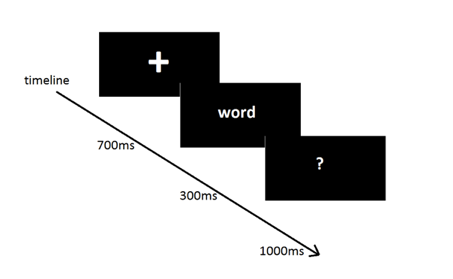
\includegraphics[width=\textwidth]{fig/experiment}
\end{figure}

\section{Source localization}

In order to source reconstruct the EEG data, the Brainstorm toolbox is used \cite{tadel2011brainstorm}. The Brainstorm toolbox is freely available under the GNU general public license. The default anatomy is based on the ICBM-152 template.

OpenMEEG BEM model is used for the forward model \cite{gramfort2014mne}. In this model, the cortex is divided into 15,000 dipoles. By merging the matrices computed from the baseline of all selected trials, the noise covariance and data covariance matrices are obtained. 

Section~\ref{source-alg} discussed different algorithm that can be used for the inverse modelling method. In this case, sLORETA is used \cite{pascual2002standardized}. sLORETA yields zero localization error. Source orientation is constrained to be orthogonal to the cortical surface. The signal-to-noise ratio (SNR) is kept at the default suggested value, which is 3. Sulci are not taken during the analysis. Brainstorm's documentation states that accurate source localization in these regions is implausible.

Using different source localization algorithms, the correctness of the procedure is verified \cite{mahjoory2017consistency}. The results are analysed by taking the average over all trials regardless of semantic features, using the four methods available in the brainstorm toolbox: wMNE, dSPM, sLORETA, and unconstrained sLORETA.

\section{Region of Interest selection}

In order to be able to focus on a very specific set of data, the delivered data only contained several regions of interest. The procedure for selecting the regions of interest starts from the source reconstructed data, obtained by using sLORETA. The current density maps were normalized with respect to a reference level in order to provide a statistical map. This statistical map is essentially the signal to noise ratio of the current estimate as a function of location. The normalized source maps are used to evaluate the significance of the data. 

The sLORETA statistical maps are averaged over all trials and activity below 75\% of the maximum activity is eliminated. This is done for both paradigms (abstract and concrete). The two obtained maps are overlapped and from this the most active regions with an estimated square size of larger than 3cm$^2$ are selected. This resulted in four regions on the inferior temporal gyrus, temporal pole, inferior frontal, and anterior orbital gyrus. Figure~\ref{experiment-2} visualizes the selected regions.

\begin{figure}[!htb]
\caption{Visualization of the Selected Brain Regions.}
\label{experiment-2}
    \centering
    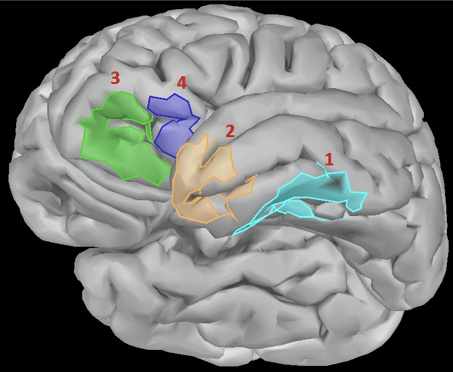
\includegraphics[width=\textwidth]{fig/experiment-2}
\end{figure}


\chapter{Evaluation}\label{evaluation}
This chapter discusses the information theoretical analysis of the dataset. The source code developed for the analysis has been implemented in the Python programming language. The actual implementation will be discussed in-depth in chapter~\ref{implementation}. 

The dataset contains the source-reconstructed data from four EEG channels. The datapoint within the dataset encompass 13 subjects. The source-reconstructed data from the abstractness and concreteness eperiment is given from 3 different regions. 

One region represents the cortical area which is active during both the abstractness and concreteness experiments. For this region, the data from both experiments are given. Another region represents the cortical area which is only active during the abstractness experiment and the final region represents the cortical area which is only active during the concreteness experiment. Finally, resting state data was available for all 3 regions.

First, this chapter will discuss the procedure for finding the amount of bins that will be used throughout the analysis. In order to be able to utilise the binning method for entropy estimation, the correct number of bins needs to be computed.

Afterwards, the main analysis is discussed. The common region which were active during both the abstractness and concreteness experiments are the main focus. Secondly, the analysis is adapted in order to analyse the different subjects  independently. Finally, an analysis was made for a comparison between the active regions and the resting state counter parts.

\section{Calculating Bin Sizes}

Section~\ref{binning} discussed the discretization of continuous data. There are multiple methods to calculate the optimal number of bins. The number of bins can be calculated empirically. This can be seen in figure~\ref{bins}. The entropy is calculated for a number of different bin sizes. Using this method, the entropy seems to converge for the bin sizes. The convergence starts from a bin size of about 100. This gives an indication for the optimal bin size.

\begin{figure}[!htb]
\caption{Entropy comparison between bin sizes}
\label{bins}
    \centering
    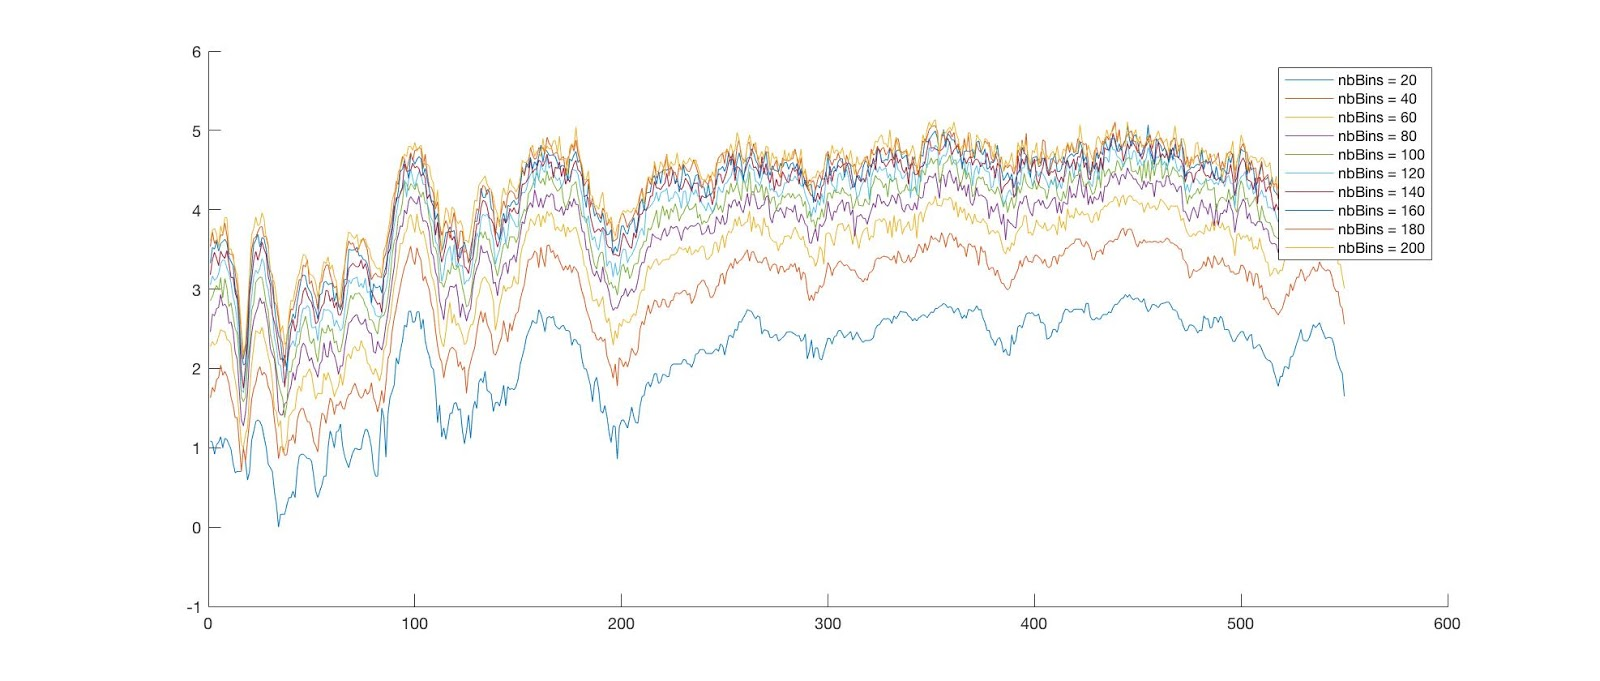
\includegraphics[width=1.2\textwidth]{fig/bins}
\end{figure}

There is also equation~\ref{binequation}. Using this equation, the optimal bin size is calculated to be 90. Both the equation and empirical method find approximately the same result. For the analysis, a bin size of 90 has been chosen. 

\section{Comparing the Common Region}\label{analysis1}

As explained before, the common region which were active during both the abstractness and concreteness experiments are the main focus. The main strength of an information theoretical approach is the measurement of mutual information. Mutual information can measure both linear and non-linear relationships. 

From the activity, we could see that some cortical areas are active during both the abstractness and concreteness experiments. Mutual information can tell us what kind of relationship there is between the abstractness and concreteness. There are several different possibilities. One theory is that the common region represents the semantic processing that is common between the abstractness and concreteness experiments.

Figure~\ref{all-channel-1} shows the results of the analysis. $Abs$, $Con$ and $Rest$ represents the information entropy through time. $Abs$ is the information entropy from the abstractness experiment. $Con$ is the information from the concreteness experiment. 

$Abs$ and $Con$ have about the same information entropy throughout time. This corresponds to the fact that this region is active and doing semantic processing. $Rest$ is the information entropy during resting state. 

\begin{figure}[!htb]
\caption{Experiment}
\label{all-channel-1}
    \centering
    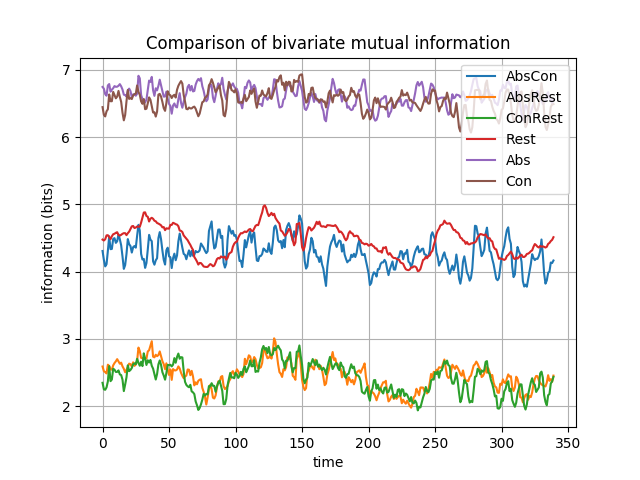
\includegraphics[width=\textwidth]{fig/all-channel-1}
\end{figure}

$AbsRest$ and $ConRest$ represent the mutual information between, respectively, abstractness and rest, and, concreteness and rest. The mutual information is much lower than the entropy from the resting state. This indicates that whatever is happening during resting state is very different from the activity during semantic processing. This is a small, but very important observation.

$AbsCon$ represents the mutual information between the abstractness experiment and the concreteness experiment. One observation is that $AbsCon$ is on an equal footing with the information entropy during the resting state. This can, wrongfully, lead to the conclusion that the only equal information between abstractness and concreteness is the activity that occurs during the resting state.

However, considering that $AbsRest$ and $ConRest$ are much lower, this conclusion cannot be made. This analysis finds that there is some mutual information between abstractness, concreteness and resting state. There is also some mutual information between the abstractness and concreteness, which is not completely caused by the resting state activity. 

Figure~\ref{venn} roughly visualizes these relationships information. There is some common information (rounded to 1 bits) between all 3 datasets. There is also some information that is unique to each of the datasets. Abstractness and concreteness share some information, which is unrelated to the resting state. This venn diagram helps visualize some results, but is very deceptive for visualizing multivariate mutual information.

There are some conclusions to be made from this. First of all, some of the semantic processing of abstractness and concreteness in the same cortical area is shared. However, it seems that the same cortical area does not compute exactly the same features during semantic processing of abstract and concrete words. 

\begin{figure}[!htb]
\caption{Venn Diagram for Information in Common Region \cite{venn}.}
\label{venn}
    \centering
    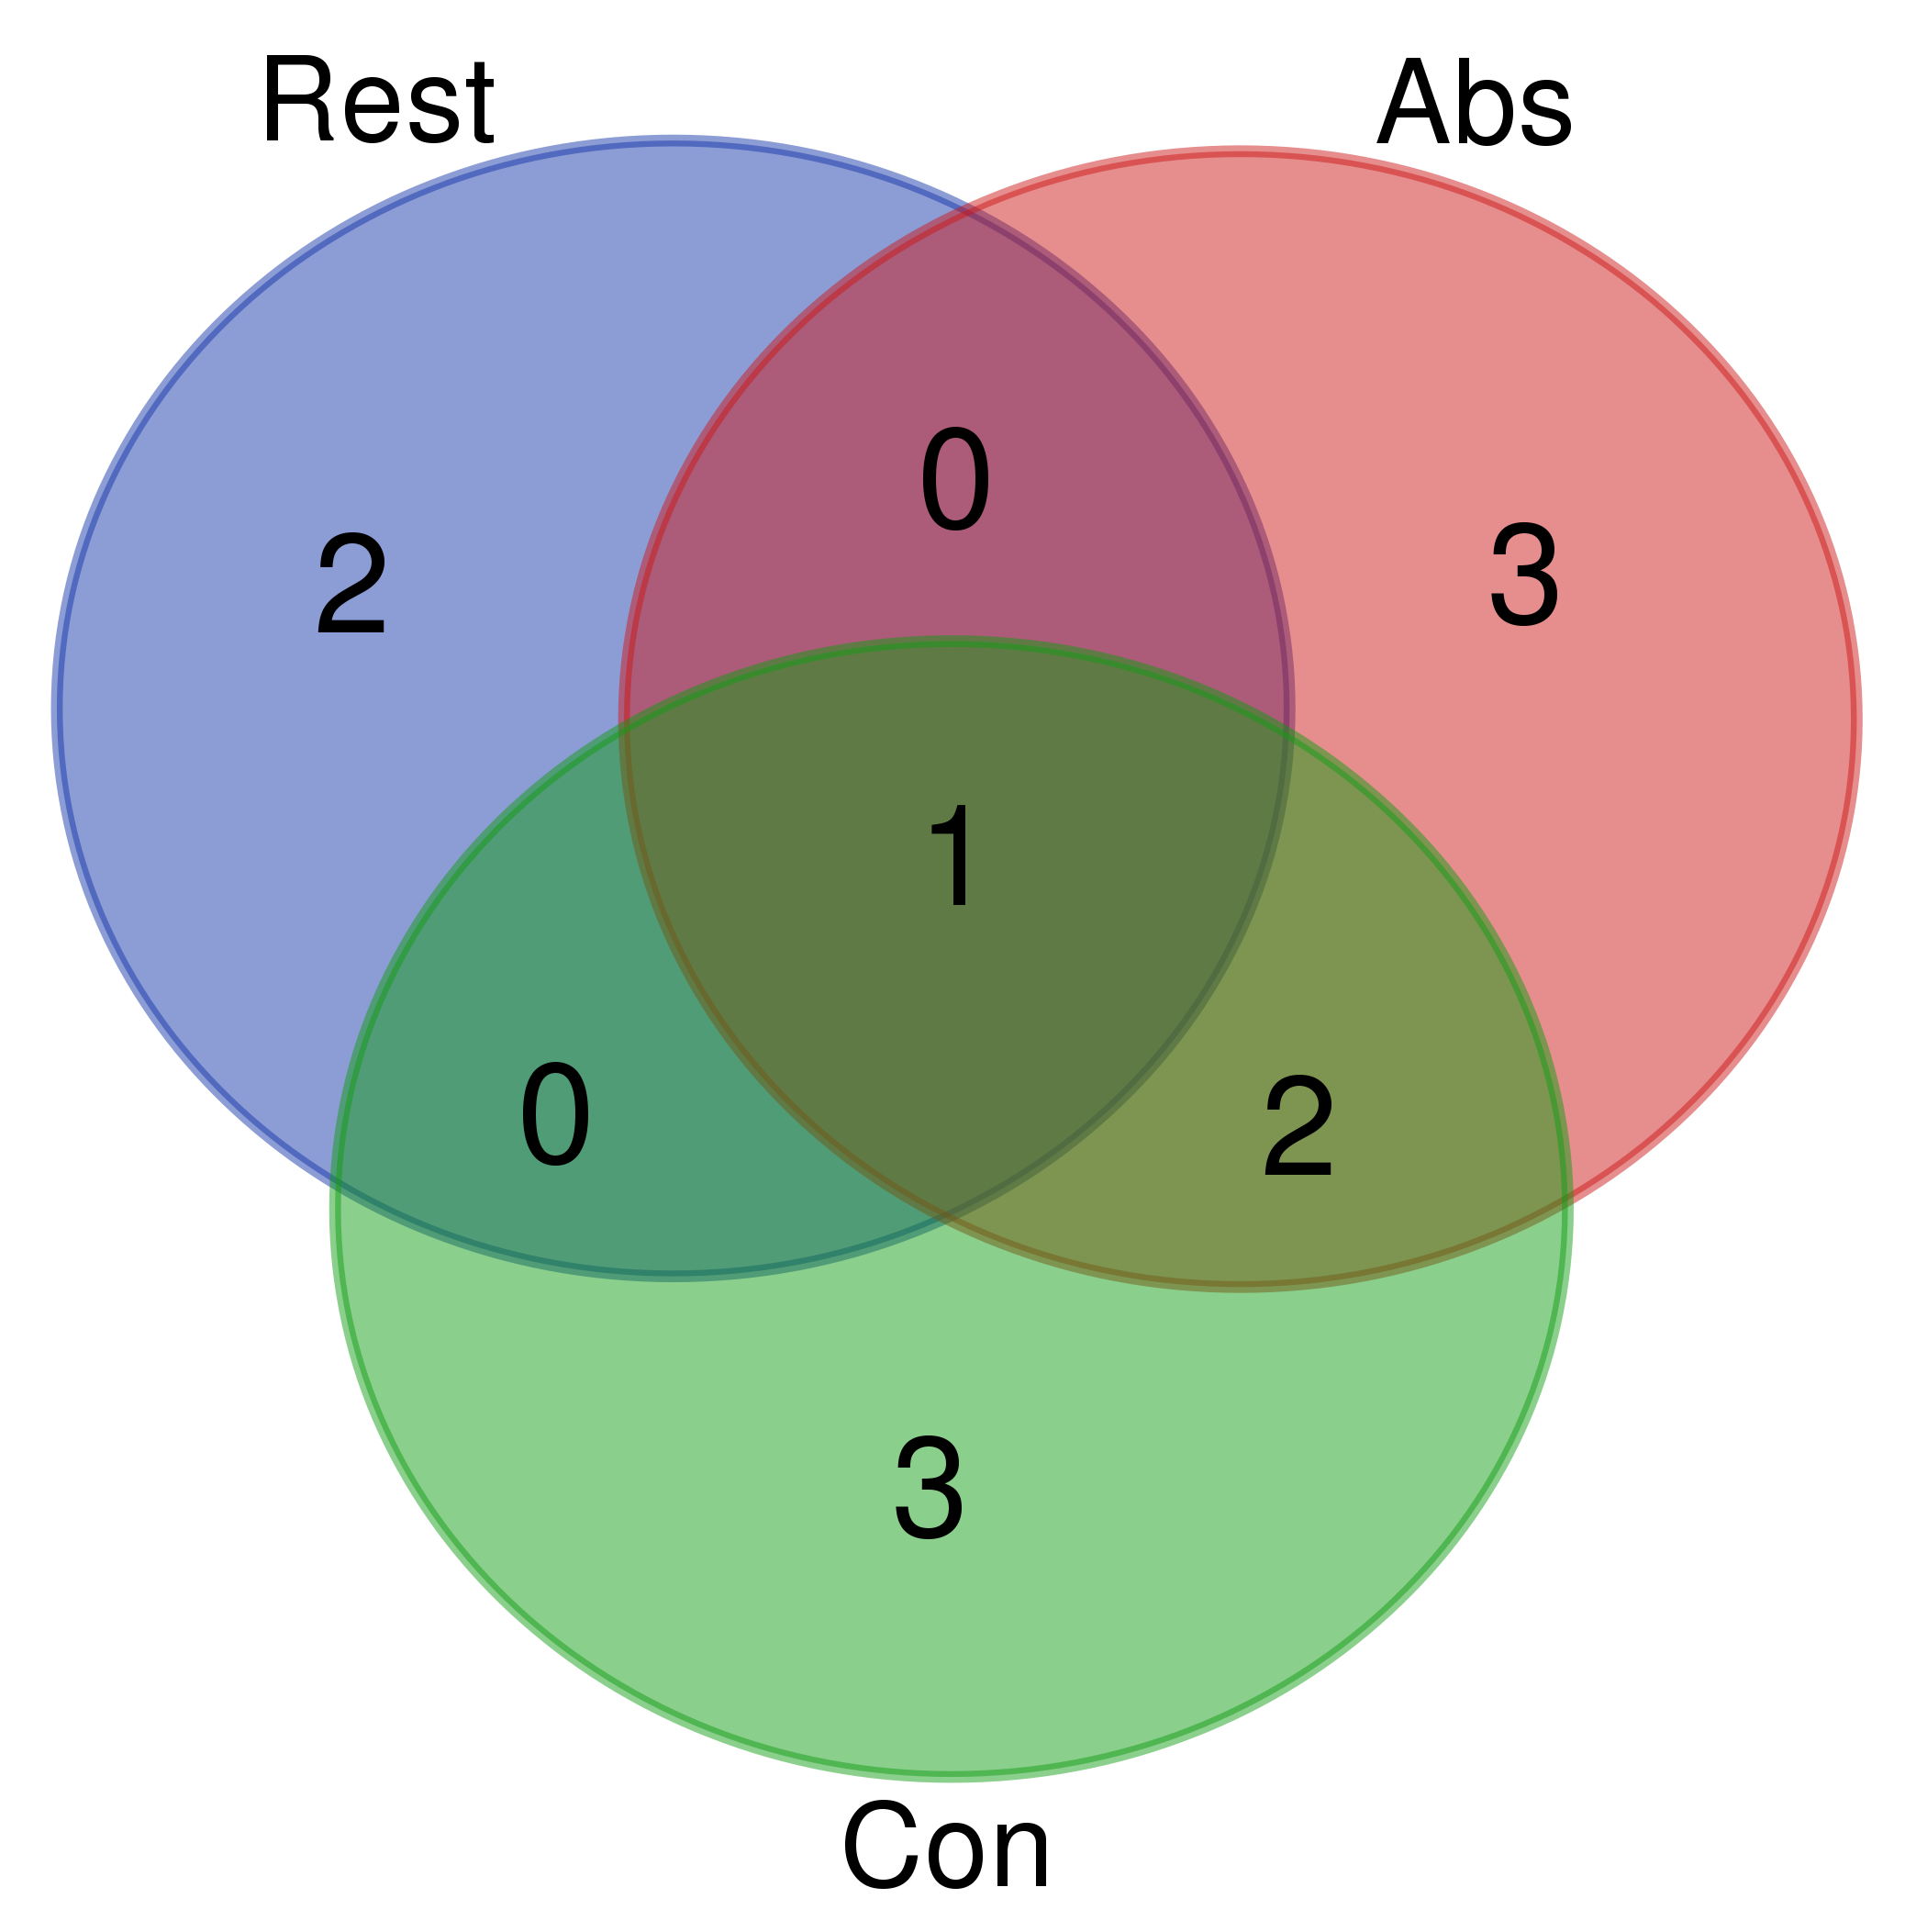
\includegraphics[width=0.8\textwidth]{fig/venn}
\end{figure}

Figure~\ref{comp-1} shows this relation expressed as percentages. About 60\% to 70\% of the activity is shared between the semantic processing of abstract and concrete words. This leaves 40\% to 30\% of the activity that is unique for the semantic processing of abstract words and for the semantic processing of concrete words.

\begin{figure}[!htb]
\caption{Comparison}
\label{comp-1}
    \centering
    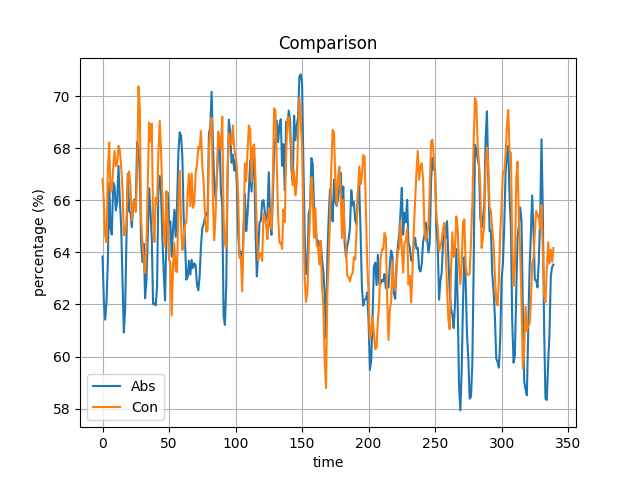
\includegraphics[width=\textwidth]{fig/comp-1}
\end{figure}

\section{Comparing the Common Region: Multivariate}\label{analysis2}

So far, bivariate mutual information has been utilised. However, there is also the multivariate mutual information. This can be used to calculate the mutual information between the abstractness, concreteness and resting state. 

Looking at figure~\ref{venn}, you would expect the multivariate mutual information to be 1 bit. However, the actual result is -1 bit, as seen in figure~\ref{mul-all-channel-1}. At first, this seems very strange. Having a negative amount of information is very counter-intuitive.

\begin{figure}[!htb]
\caption{Multivariate Experiment}
\label{mul-all-channel-1}
    \centering
    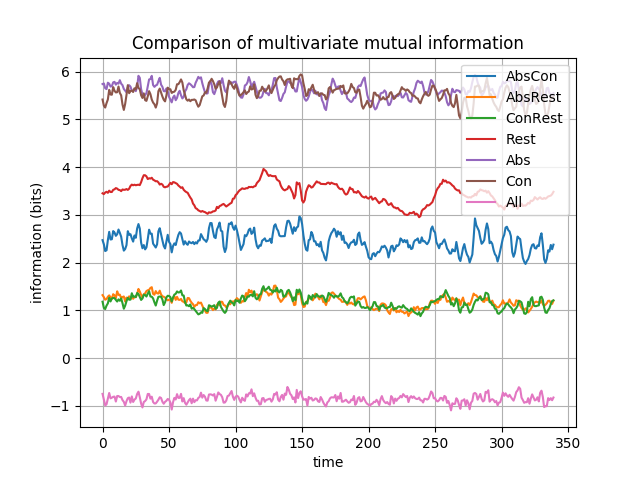
\includegraphics[width=\textwidth]{fig/mul-all-channel-1}
\end{figure}

Looking at the equation that is used for the multivariate mutual information, we get:

\begin{equation}
I(Abs, Con, Rest) = I(Abs, Con) - I(Abs, Con | Rest)
\end{equation}

Looking at figure~\ref{mul-all-channel-1}, we can see that $I(Abs, Con)$ has a value between 2 and 3 bits of information. However, $I(Abs, Con | Rest)$ is a bit more difficult. This can also be written as a sum of entropies:

\begin{equation}
I(Abs, Con | Rest) = H(Abs,Rest)+H(Con,Rest)-H(Abs, Con, Rest)-H(Rest)
\end{equation}

The deceptive point is that the joint entropy $H(Abs, Con, Rest)$ isn't as large as the venn diagram makes it look. The result is that $I(Abs, Con | Rest) > I(Abs, Con)$, which causes a negative multivariate mutual information. 

Negative multivariate mutual information indicates a synergy. Figure~\ref{common} shows a graphical model detailing this. $Z$ and $Y$ represent $Abs$ and $Con$, while $X$ represents $Rest$. $Rest$ causes a stronger dependency between $Abs$ and $Con$, than without $Rest$. This shows that multivariate mutual information is quite difficult to interpret.

\begin{figure}[H]
\caption{Multivariate Mutual Information Synergy}
\label{common}
    \centering
    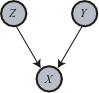
\includegraphics[]{fig/common}
\end{figure}
    

\section{Per Subject Comparison}

An per-subject analysis has also been performed. With a per-subject analysis, we can see whether results would vary between different subjects and whether there are different conclusions to be made.

Figure~\ref{all-trials} shows the analysis from section~\ref{analysis1} executed on a single subject. The figure looks very similar to figure~{all-channel-1}. This reaffirms the conclusion on a per-subject basis.

\begin{figure}[!htb]
\caption{Comparison for Subject 1}
\label{all-trials}
    \centering
    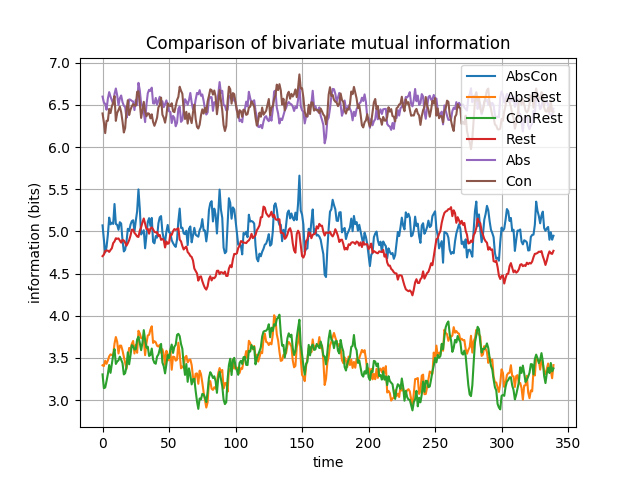
\includegraphics[width=\textwidth]{fig/subject1_alltrials_all-channel-1}
\end{figure}

\subsection{Effect of Trials Used}

Another interesting avenue to pursue was analysing the effect of the amount of trials used within information theoretical equations. In other words, how much data do we need in order to get decent results. We expected that information theory would still deliver good results, even with relatively few data.

Several additional analyses were performed. Each analysis used a different amount of trials. The complete dataset contains 3404 datapoints, with an average of 262 datapoints per subject (per timepoint). With binning being done with 90 bins, this means that there are about 3 datapoints in each bin. 

In order to see the effect of the amount of datapoints that are used, the information theoretical analysis was performed with 10, 40, 80 and 100 datapoints. 

Figure~\ref{10-trials} shows the result from only using 10 datapoints. With 90 bins, most bins are completely empty. Due to this, the computed information entropy is very inaccurate. 

\begin{figure}[!htb]
\caption{Comparison for Subject 1 - 10 datapoints}
\label{10-trials}
    \centering
    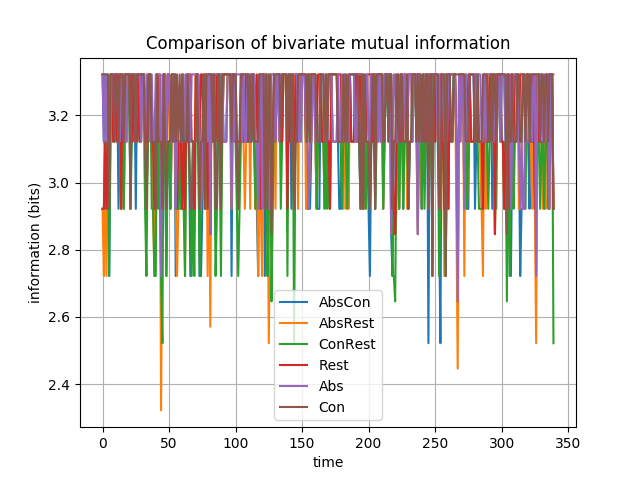
\includegraphics[width=\textwidth]{fig/subject1_10trials_all-channel-1}
\end{figure}

Figure~\ref{40-trials} shows the result from only using 40 datapoints. In this case, the result starts becoming more accurate.

\begin{figure}[!htb]
\caption{Comparison for Subject 1 - 40 datapoints}
\label{40-trials}
    \centering
    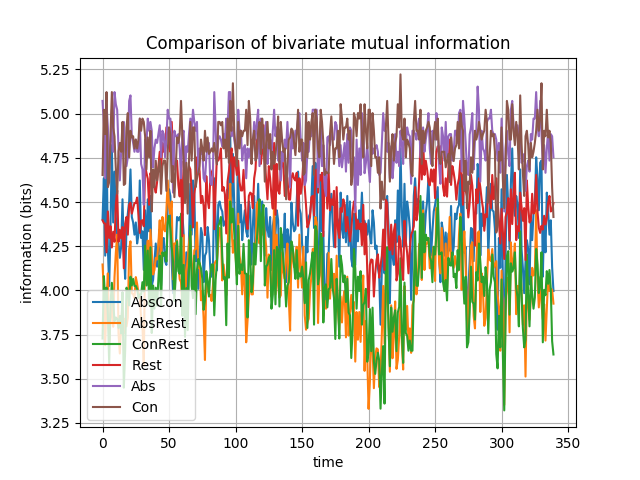
\includegraphics[width=\textwidth]{fig/subject1_40trials_all-channel-1}
\end{figure}

Figure~\ref{80-trials} shows the result from using 80 datapoints. With 80 datapoints, nearly every bin should be filled. From this point, the resolution starts becoming much more accurate. 

\begin{figure}[!htb]
\caption{Comparison for Subject 1 - 80 datapoints}
\label{80-trials}
    \centering
    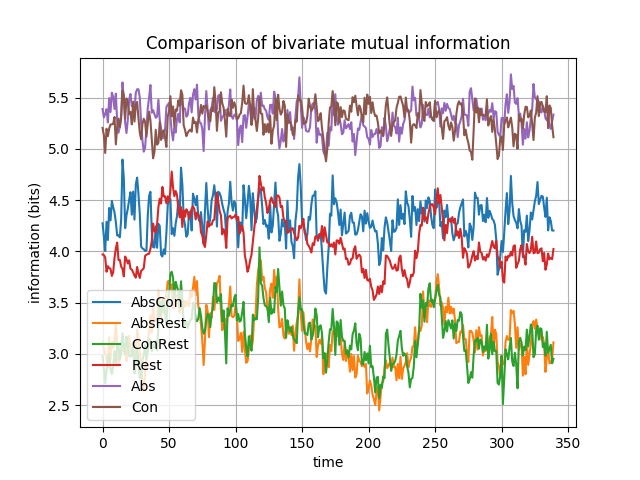
\includegraphics[width=\textwidth]{fig/subject1_80trials_all-channel-1}
\end{figure}

Figure~\ref{100-trials} shows the result from using 100 datapoints. The resolution increases yet again. However, the new details that are visible in the graph do not cause more conclusions or results to be drawn. 

This analysis shows that, if not enough data is available, information theoretical equations cannot reliably be used. For the 10 and 40 datapoint analyses, this is clearly shown. However, the 80 and 100 datapoint analyses show that even with relatively few datapoints, relative to the amount of bins used, the resolution is already quite clear.

\begin{figure}[!htb]
\caption{Comparison for Subject 1 - 100 datapoints}
\label{100-trials}
    \centering
    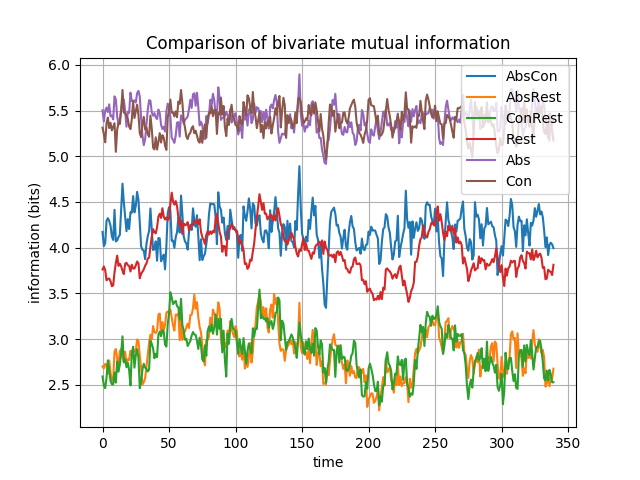
\includegraphics[width=\textwidth]{fig/subject1_100trials_all-channel-1}
\end{figure}



\chapter{Implementation}\label{implementation}
\section{Language}

\section{Data Conversion}

\chapter{Related Work}\label{related}
This thesis specifically focussed on information theoretical measures for brain connectivity. However, there are several other methods which can be used to measure brain connectivity.

One method especially of interest is granger causality. 

\section{Granger Causality}



\chapter{Future Work}\label{future-work}
Even though this thesis has come to a close, there are still many opportunities to take and avenues to explore. The results from this thesis shows that there is a lot of promise for an information theoretical approach for EEG source-reconstructed data. 

\section{Directed Information}

In section~\ref{directed-information}, directed information was described. This is a very interesting algorithm that can lead to many interesting results. Directed information allows information flow between two processes to be calculated. 

This is especially useful for information flow and connectivity. In the case of the source-reconstructed EEG data used in this thesis, directed information can be used to compute the flow of information between different regions in the brain. 

This could be useful to further investigate what the activity within the common region (between abstractness and concreteness) means. One of the possible questions could be, does the flow of information start within the common region, or does it start in the seperate regions and then flow to the common region.

\begin{equation}
I(X^n \rightarrow Y^n) = \sum^{n}_{i=1}I(X^i, Y_i | Y^{i-1})
\end{equation}

\section{Open Source Connectivity Package}
The implementation has been described in-depth in chapter~\ref{implementation}. This was explained in-depth for multiple purposes. Being able to use the source code to develop an open-source connectivity package is one of the main reasons. 

Currently, the implementation is not in a state where it can be released as an open-source toolbox. Other connectivity measures need to be added to the source code and the current implementation needs to be cleaned-up. 

\section{Comparison with Granger Causality}

In this thesis, the information theoretical equations have not been compared to other connectivity measures. Most notably, the granger causality could be compared against. 

\section{Multivariate Mutual Information Alternatives}

Multivariate mutual information can be difficult to interpret. This is especially the case when the multivariate mutual information is negative. The main cause is that multivariate mutual information heavily shows synergies and redundancies.

However, the multivariate mutual information described in this thesis, interaction information, is not the only generalisation for mutual information. There is also total correlation and dual total correlation. These are non-negative generalizations of mutual information.

Total correlation measures the divergence of the joint entropy to the independent entropies.

\begin{equation}
C(X^1,...,X^n) = [\sum^{n}_{i=1}H(X^i)] - H(X^1,...,X^n)
\end{equation}

Dual total correlation is bounded by the joint entropy.

\begin{equation}
D(X^1,...,X^n) = H(X^1,...,X^n) - \sum^{n}_{i=1}H(X^i | X^1,...,X^{i-1},X^{i+1},...,X^n)
\end{equation}

Both of these methods are rarely used within the context of computational neuroscience. Due to the strength of being a non-negative generalizations of mutual information, the measure is easier to interpet. It would therefore be interesting to see how useful total correlation and dual total correlation can be when dealing with EEG source-reconstructed data.

\chapter{Conclusion}\label{conclusion}
The main goal of this thesis is to apply information theoretical measures of brain connectivity to a high density EEG source-reconstructed dataset. Information theoretical algorithms are becoming more and more utilised within the field of computational neuroscience. 

Information theoretical algorithms are model-free and probability based. They make no assumptions on what kind of distribution the data has. This makes information theoretical algorithms very versatile and an excellent tool to measure connectivity.

This thesis mainly focussed on 2 different information measurements. The first measurement is bivariate mutual information. The second measurement is a generalisation of mutual information, called multivariate mutual information or interaction information.

The provided EEG dataset was produced by an experiment resolving around semantic processing. More specifically, the experiment compared the brain activity between the semantic processing of concrete words and abstract words. The provided EEG dataset had already been source-reconstructed.

One cortical area of interest was an area that was active during both semantic processing of abstract and concrete words. Analysis showed that the actual activity in this area differed between the semantic processing of abstract and concrete words.

The implementation has been carefully developed such that the source code can be used in open-source projects. In the future, we want to further develop the implementation so it can be released as an open-source connectivity package which can be used by other scientists. 

In conclusion, an analysis of a high density EEG dataset has been computed and an implementation has been developed. The implementation provides a platform for further information theoretical analysis and research.  

% \appendixpage*
% \appendix

\backmatter

% The bibliography comes after the appendices.
% You can replace the standard "abbrv" bibliography style by another one.
\bibliographystyle{abbrv}
\bibliography{bib/main}
\nocite{*}

\end{document}
